% GENERATED FILE. DO NOT EDIT.
% Source: ../manuscript.md via latex/manuscript.tex
% Build: python build_latex.py
\documentclass[11pt]{article}
\usepackage[margin=1in]{geometry}
\usepackage[T1]{fontenc}
\usepackage[utf8]{inputenc}
\usepackage{amsmath,amssymb}
\usepackage{graphicx}
\usepackage{booktabs}
\usepackage{tabularx}
\usepackage{array}
\usepackage{hyperref}
\newcolumntype{Y}{>{\raggedright\arraybackslash}X}
\title{Diagnostic Weak-Label Hawkes Validation for Event-Driven Crypto Futures}
\author{Joohyoung Jeon \\ Korea University \\ Seoul, Republic of Korea}
\date{}

\begin{document}
\maketitle

\begin{abstract}
We build an auditable diagnostic layer for event-driven weak labels in crypto futures microstructure. The framework maps external event timestamps to activation rows, decomposes market response into persistent price impact and liquidity recovery, assigns PPI-primary/RR-validator labels, and asks whether the resulting classes imply different bucketed exogenous Hawkes decay in subsequent buy/sell order flow. On BTC/ETH Binance futures, 95 primary macroeconomic candidates yield 380 activation attempts, 60 activation-positive rows, and 46 computed labels (under the schema names Information(schema) and Noise(schema)). We frame the contribution around three structural barriers: PPI/RR semantic misalignment (30 of 34 computed Information(schema) rows, or 88\%, are PPI-persistent but RR-recovered, outside the adverse-selection signature), event-family confounding (the cohort-level class contrast collapses to a small number of release-batch clusters per cohort), and bucket-level identification limits at the one-second trade-bucket / 600-second horizon. Consistent with these barriers, all six M0/M1/M2 Hawkes fits converge but nominal diagnostic p-values do not reject pooled-exogenous M0 (BTCUSDT p = 0.666; ETHUSDT p = 0.999), and the fitted decay rates do not support the diagnostic hypothesis directionally. A two-held-out-event small-sample materiality check places M1 and M0 within the 5.0-nat threshold; a release-batch dependence audit records missing per-cluster likelihood contributions; and a 108-point threshold-sensitivity audit finds label composition stable across the grid. An endogenous-only diagnostic shows the pooled-exogenous layer is not justified by AIC/BIC in BTCUSDT and is criterion-dependent in ETHUSDT, so BTCUSDT's non-rejection is partly an exogenous-identification limitation. The artifacts are an input contract for later prediction and execution research; no downstream performance result is reported here.

\end{abstract}

\section{Introduction}

External-event systems in crypto derivatives markets face a labeling problem before they face a prediction problem. Scheduled macroeconomic announcements, exchange notices, and other timestamped public events can coincide with price displacement, spread changes, missing market-data coverage, or overlapping release batches. A useful event catalog therefore needs more than event timestamps: it needs an auditable way to record which events generated observable market responses, which responses are labelable, and which cases remain ambiguous, confounded, or insufficiently covered.

Existing literatures address adjacent parts of this design. Event studies formalize external timestamps and event windows \cite{MacKinlay1997EventStudies,AndersenEtAl2003MacroAnnouncements}. Microstructure work connects order-book events, trade informativeness, and price impact \cite{ContKukanovStoikov2014OrderBookEvents,CampigliBormettiLillo2023PriceImpact}. Weak-supervision systems provide a vocabulary for noisy rules, abstentions, and conflicts \cite{RatnerEtAl2017Snorkel}. Hawkes models provide a statistical framework for self-exciting order-flow dynamics \cite{BacryMastromatteoMuzy2015HawkesFinance}. The missing empirical contract is an end-to-end diagnostic layer that turns external event reactions into weak Information(schema)/Noise(schema) labels and then tests whether those labels contain detectable order-flow persistence content.

This paper builds that diagnostic layer for BTC/ETH Binance futures. The first stage maps external events to market-data windows and records activation outcomes. The second stage measures persistent price impact and liquidity recovery, combines their verdicts into PPI-primary/RR-validator weak labels, and preserves abstention, confounding, and confidence states. The third stage fits a class-specific exogenous Hawkes model suite as a validation layer. The labels are diagnostic inputs to the Hawkes comparison, not ground truth and not outputs of the Hawkes model.

The empirical result is a boundary condition rather than a positive class-specific decay result. In the expanded-universe diagnostic run, 95 primary macroeconomic candidates yield 380 activation attempts, 60 activation-positive rows, and 46 computed Information(schema)/Noise(schema) labels after coverage and label-quality filters. All six M0/M1/M2 fits converge across the BTCUSDT main cohort and ETHUSDT robustness cohort, but the M1-vs-M0 likelihood-ratio diagnostic does not reject the pooled-exogenous M0 specification. The neutral validation audits preserve that boundary: the out-of-sample materiality audit classifies M1 and M0 as materially similar, the release-batch dependence audit records that per-cluster likelihood contributions are not exported by the current Hawkes-fit output limitation rather than an adjusted p-value, and the fixed-surface threshold-sensitivity audit reports label-composition stability rather than threshold calibration.

The paper's contribution is therefore primarily diagnostic. We frame the contribution around three structural barriers that the validation pipeline identifies and characterizes, plus a reproducible artifact contract on which later work can build:

\begin{enumerate}
\item A versioned weak-label validation framework that separates activation, PPI/RR diagnostics, confidence states, abstention, confounding, and the bucketed exogenous Hawkes validation layer, with append-only run directories and hash-addressed manifests.
\item A first-pass BTC/ETH macro-event artifact set whose computed label sample is explicit about coverage loss, activation selectivity, and label-quality filters, and whose schema labels Information and Noise are defined as PPI-persistent and PPI-transient/RR-recovered descriptors rather than as economic information content in the \cite{Kyle1985ContinuousAuctions} and \cite{GlostenMilgrom1985BidAsk} sense.
\item Quantitative evidence for three structural barriers that any future event-driven crypto weak-label study in this regime must address: (i) PPI/RR semantic misalignment, where 30 of 34 computed Information(schema)-class rows (88\%) arise from PPI-persistent but RR-recovered cases that fall outside the spread-stress signature predicted by adverse-selection theory; (ii) event-family confounding, where the computed labels are nearly deterministic by macro-release family and the M0/M1 comparison effectively contrasts CPI events against Labor / Retail / ISM events rather than two within-family classes; and (iii) bucket-level identification limits, where the one-second trade bucket and the 600 s validation horizon constrain the identifiable exogenous decay range and place at least one cohort estimate near the bucket-aliasing edge.
\item Neutral validation outcomes that document out-of-sample materiality, the current artifact boundary for dependence-aware inference, and fixed-surface threshold stability, all read as evidence consistent with the three barriers rather than as a standalone non-rejection result.
\end{enumerate}

We position the paper as the Phase 1 validation layer of a validation-to-prediction-to-decision program. Later work can use the event universe, activation rows, label rows, confidence fields, abstention statuses, and Hawkes diagnostics as inputs for ex-ante event-quality prediction, real-time filtering, or execution-policy design. This paper does not estimate a downstream predictor, deploy a real-time filter, or report an execution result.

The remainder of the paper is organized as follows. Section 2 reviews the event-study, microstructure, weak-supervision, and Hawkes-process literatures. Sections 3 and 4 define the weak-label and Hawkes validation methods. Section 5 describes the computational reproducibility contract. Section 6 reports the empirical funnel, Hawkes comparison, neutral validation audits, and diagnostic patterns. Section 7 discusses limitations and the requirements for a future validation expansion. Section 8 describes how the validation outputs define inputs for later prediction and decision layers. Section 9 concludes.

\section{Related Work}

This paper connects four strands of prior work: event studies, high-frequency market microstructure, weak supervision, and Hawkes-process modeling. The connection is methodological. Event studies define the external timestamp and the counterfactual window; microstructure models define the observable market response; weak supervision provides a vocabulary for noisy and abstaining label rules; and Hawkes processes provide a validation layer for testing whether labels correspond to different subsequent order-flow dynamics.

\subsection{Event Studies and Market Reactions}

The event-study literature provides the basic empirical grammar for this setting: a dated public event is paired with pre-event and post-event windows, and the market response is measured relative to a baseline \cite{MacKinlay1997EventStudies}. High-frequency studies of macroeconomic announcements show that scheduled news can affect prices over very short horizons, making timestamp quality and event-window construction central to the empirical design \cite{AndersenEtAl2003MacroAnnouncements}. Related jump-test work formalizes the distinction between continuous variation and discontinuous high-frequency moves, which is relevant when an event reaction appears as a localized market discontinuity rather than as a slow drift \cite{BarndorffNielsenShephard2006Jumps}.

The present framework adopts the event-window structure but changes the response variable. Instead of treating the event study as a single abnormal return exercise, it measures whether the event produces a persistent price impact and whether liquidity stress subsequently recovers. This distinction is important for crypto futures because trading is continuous, liquidity conditions change quickly, and a timestamped macro release may affect price and order-book state on different horizons.

\subsection{Crypto Microstructure and Order Flow}

Market microstructure studies motivate the two components used in the weak label. Order-book event flow and order-flow imbalance are directly connected to short-horizon price impact \cite{ContKukanovStoikov2014OrderBookEvents}, while time-varying price-impact estimates help separate trades with higher information content from trades whose effects are more transient \cite{CampigliBormettiLillo2023PriceImpact}. Bitcoin high-frequency jump evidence further motivates treating crypto markets as a setting where discontinuous responses are empirically plausible \cite{ScailletTreccaniTrevisan2020BitcoinJumps}. High-dimensional limit-order-book Hawkes models also show that order-book state and event arrivals can be modeled jointly, but at the cost of a substantially larger calibration problem \cite{LuAbergel2018HighDimensionalLOBHawkes}.

This paper uses these ideas in a reduced-form way. The persistent price-impact index is intended to capture whether the event leaves a lasting mid-price displacement. The recovery ratio is intended to capture whether spread dislocation normalizes after the event. The two quantities are related but not interchangeable: a market can reprice without immediate liquidity recovery, and liquidity can normalize without a durable price move. The empirical label policy therefore records disagreement between price impact and recovery rather than forcing the two measurements into a single hidden score.

\subsection{Weak Supervision and the Information/Noise Naming Caveat}

The labels in this study are weak labels, not human-verified ground truth. Weak-supervision systems formalize labeling functions, abstentions, conflicts, and operational label pipelines \cite{RatnerEtAl2017Snorkel,BachEtAl2019DryBell}. That vocabulary is useful for financial event classification because many event reactions are intrinsically ambiguous: multiple announcements can occur at the same timestamp, market data can be missing around the event, and different microstructure measurements can imply different interpretations.

The pipeline therefore treats label generation as an auditable rule system. Events are recorded under the schema names Information and Noise, but they can also abstain because of confounding, insufficient horizon data, or disagreement between diagnostic signals. Recent work on Hawkes processes under label noise highlights why this distinction matters: noisy event labels can alter downstream point-process inference, so label uncertainty should be preserved rather than hidden \cite{TanEtAl2024RobustDeepHawkesLabelNoise}. In this paper, the Hawkes model is not used to create labels; it is used as a validation layer after weak labels have been generated.

We adopt a deliberate naming caveat. Classical microstructure theory predicts that an information event leaves persistent spread widening because liquidity providers price-protect against asymmetric information \cite{Kyle1985ContinuousAuctions,GlostenMilgrom1985BidAsk}; under that prediction, true information events should appear as PPI-persistent and RR-stressed cases. The empirical PPI-primary/RR-validator rule used here instead labels rows as Information whenever PPI is information-side, even when the RR validator records spread recovery. The schema names Information and Noise should therefore be read as versioned identifiers for PPI-persistent and PPI-transient/RR-recovered rows, not as economic information content in the Kyle/Glosten-Milgrom sense. The first structural barrier reported in Section 6 quantifies the gap between the schema labels and the theoretical prediction.

\subsection{Hawkes Processes for Financial Events}

Hawkes processes are widely used in finance to model clustering, excitation, and endogeneity in event arrivals \cite{BacryMastromatteoMuzy2015HawkesFinance}. In cryptocurrency markets, Hawkes-style models have been used to quantify endogeneity and reflexivity \cite{MarkSilaWeber2022CryptoEndogeneity} and to model limit-order-book dynamics for forecasting and state-dependent behavior \cite{CestariEtAl2023CryptoHawkesLOB,RaffaelliEtAl2026BitcoinHawkesLOB,MorariuPatrichiPakkanen2022StateDependentHawkes}. Marked and state-dependent variants provide ways to condition excitation on event type or market state \cite{LeeSeo2017MarkedHawkes,MorariuPatrichiPakkanen2022StateDependentHawkes}.

The model used here is deliberately narrower than a full high-dimensional limit-order-book Hawkes model. It treats buy/sell trade-flow arrivals as the endogenous point process and external weak-labeled events as exogenous marks. The comparison asks whether class-specific exogenous decay improves fit relative to a pooled-exogenous specification. This framing turns Hawkes estimation into a test of weak-label usefulness: if the schema labels contain detectable order-flow persistence content, a class-specific model should improve the likelihood enough to justify its additional parameters.

\section{PPI/RR Weak Label Framework}

The weak-label layer maps an activated external event into a label row. Its input is not the raw event universe directly, but an activation row whose short-window response has already passed the empirical activation gate. This gate separates event selection from label interpretation: an event must first produce an observable short-horizon market response before the longer-horizon PPI/RR label rules are evaluated.

Activation is defined on one-second market buckets anchored at the event time $\tau_k$. The empirical activation rule uses the same price and order-flow thresholds as the strict semantic rule, but allows sparse pre-event baseline coverage when the observed-row coverage ratio is at least 0.99. This tolerance does not forward-fill or interpolate missing one-second rows. It only permits baseline statistics to be computed from observed adjacent bucket pairs. The activation output is therefore an evidence gate, not a label.

For each activated event, the label rule evaluates two diagnostics. The price-impact persistence index is

\[
\mathrm{PPI}_k(H) =
\frac{\left|\log m(\tau_k + H)-\log m(\tau_k - 1s)\right|}
     {\hat{\sigma}^{label}_{pre,k}(H)},
\]

where $m(t)$ is the one-second mid price and $H=30$ minutes in the empirical rule. The denominator is a pre-event long-horizon return scale computed over a 24-hour lookback window using overlapping 30-minute returns sampled at one-minute stride. PPI is interpreted as a permanence proxy: values at or above the information threshold produce an Information-side verdict, values at or below the noise threshold produce a Noise-side verdict, and intermediate values are undetermined. The empirical first-pass rule uses thresholds 2.0 and 0.75, respectively.

The liquidity-side diagnostic is the recovery ratio

\[
\mathrm{RR}_k(H_R) =
\frac{\mathrm{spread}(\tau_k + H_R)}
     {\mathrm{spread}(\tau_k - 1s)},
\]

with $H_R=30$ minutes. A ratio near one indicates that the spread has recovered toward its pre-event level, while a larger ratio indicates persistent liquidity stress. The empirical rule maps $\mathrm{RR}\geq1.25$ to an Information-side verdict and $\mathrm{RR}\leq1.05$ to a Noise-side verdict; intermediate ratios are undetermined. As with PPI, missing or numerically invalid evidence yields an insufficient-horizon state.

The strict rule computes a label only when PPI and RR agree. The empirical rule used for the reported results instead treats PPI as the primary label decision and RR as a validator. If PPI is information or noise, the label is computed from the PPI verdict. Agreement with RR yields \texttt{High} confidence; disagreement yields \texttt{Low} confidence and remains visible in the label row. If PPI is undetermined, the row abstains as ambiguous. This policy is motivated by the empirical observation that PPI/RR agreement is not common in the macro-TE sample, and that discarding all disagreement removes most otherwise usable activation evidence.

The label rule also applies a confounding scan before PPI/RR computation. The scan searches for other candidate or tier-2 events in $[\tau_k-5\mathrm{min},\tau_k+60\mathrm{min}]$. Cross-source events in this window cause a confounded abstention. Same-source same-timestamp macro releases are treated as dependent batch context rather than as unrelated confounders; this prevents scheduled release bundles from being incorrectly classified as mutual contamination. The resulting label row preserves the final status, PPI/RR verdicts, confidence, confounding flag, and deterministic feature snapshot identity for downstream diagnostics.

\section{Class-Specific Exogenous Hawkes Framework}

The Hawkes layer is a validation model for the weak labels. It does not create or revise label rows. The target process is a two-dimensional point process over aggressive buy and sell trade arrivals. In the current production data adapter, one nonzero net-signed one-second trade bucket is represented as one point event; we therefore refer to the model as a bucketed exogenous Hawkes diagnostic rather than as a tick-level Hawkes model. The validation horizon is $H = 600$ seconds. Together with the one-second bucket, this fixes the identifiable range of the exogenous decay rate at roughly $\beta_{\min} \approx 1/H \approx 1.7 \times 10^{-3}$/s on the lower end and at most $\beta_{\max} \approx \log(2)/1\,\mathrm{s} \approx 0.69$/s on the upper end; estimates near the upper edge sit close to the bucket-aliasing limit and should be read with that caveat in mind. The bucket-granularity approximation is reported as part of the data contract and is not interpreted as tick-level trade reconstruction.

For target dimension $q\in\{\mathrm{buy},\mathrm{sell}\}$, the shared endogenous component is

\[
\lambda_q(t)=\mu_q+
\sum_r\sum_{t_i^r<t} a_{rq}\exp[-b_{rq}(t-t_i^r)]
+x_q(t),
\]

where $r$ indexes the two order-flow dimensions and $x_q(t)$ is the exogenous event component. Including the endogenous component is necessary because trade arrivals cluster even without external events; the exogenous term should not absorb ordinary buy/sell self- and cross-excitation.

The model suite compares three exogenous specifications. In M0, Information(schema) and Noise(schema) labels share one pooled exogenous decay:

\[
x_q^{M0}(t)=
\sum_k \eta_{q,p}\exp[-\beta_p(t-\tau_k)]\mathbf{1}\{0<t-\tau_k\leq H\}.
\]

In M1, the exogenous decay is class-specific:

\[
x_q^{M1}(t)=
\sum_k \eta_{q,g_k}\exp[-\beta_{g_k}(t-\tau_k)]
\mathbf{1}\{0<t-\tau_k\leq H\},
\quad g_k\in\{\mathrm{Information},\mathrm{Noise}\}.
\]

In M2, only Information(schema) exogenous impulses are retained; Noise(schema) labels are excluded from the exogenous term and remain in coverage diagnostics. The validation horizon is $H=600$ seconds in the reported empirical rule, and all exogenous marks are unit marks.

The H3 observation adapter deduplicates label rows by (event\_id, symbol, venue, label) and stitches each deduplicated event as its own 600-second validation segment, with one unit impulse at each segment-start. Same-timestamp release bundles (e.g. CPI headline / core / MoM / YoY) therefore inflate the number of validation segments contributed to the stitched observation rather than the impulse amplitude on a shared time axis. Section 6.4 quantifies the multiplicity at the deduplicated-event level (24 -\textgreater{} 12 -\textgreater{} 8 for BTCUSDT main, 22 -\textgreater{} 11 -\textgreater{} 6 for ETHUSDT robustness). Section 6.7 reports the input-unit audit. A genuine batch-level mark-aggregation refit, which would reduce same-timestamp segments to a single segment with a chosen trade-window convention, requires changing the segment-construction contract and is deferred to the future-validation expansion (Section 7).

The likelihoods reported below should therefore be read as segment-stitching diagnostics, not as a calendar-time Hawkes likelihood over independent release moments; same-timestamp bundles can contribute repeated 600-second market-flow segments under the current observation contract.

The diagnostic hypothesis is that Information(schema) events should have a more persistent exogenous footprint than Noise(schema) events. With the exponential kernel, this corresponds to $\beta_{\mathrm{Information}} < \beta_{\mathrm{Noise}}$, or equivalently $\log(2)/\beta_{\mathrm{Information}} > \log(2)/\beta_{\mathrm{Noise}}$. The empirical comparison therefore asks whether M1 improves fit relative to M0 enough to justify its additional class-specific parameters.

Parameters are estimated by maximum likelihood with positive intensities, amplitudes, and decay rates. The implementation uses empirical-rate initialization, analytic gradients for the log-parameterized objective, and L-BFGS-B optimization. The observation is split chronologically into in-sample and out-of-sample portions; random splitting is not used because event arrivals and market regimes are serially dependent. The reported tables include in-sample log likelihood, out-of-sample log likelihood, AIC/BIC differences, fitted decay rates, half-lives, and fit status. The BIC calculations use the computational point-process event count in the stitched in-sample stream ($n=1{,}920$ for BTCUSDT main and $n=1{,}760$ for ETHUSDT robustness), not the smaller release-batch cluster counts used for inferential calibration.

M1 is compared with M0 using a likelihood-ratio diagnostic with degrees of freedom equal to the parameter-count difference in the fitted model. In the reported empirical fits this difference is three. Concretely, in the exogenous component M0 has three parameters, $\eta_{\mathrm{buy},p}$, $\eta_{\mathrm{sell},p}$, and $\beta_p$, while M1 has six, $\eta_{\mathrm{buy},I}$, $\eta_{\mathrm{sell},I}$, $\eta_{\mathrm{buy},N}$, $\eta_{\mathrm{sell},N}$, $\beta_I$, and $\beta_N$; the resulting parameter-count difference is therefore three. We emphasise that M1 vs M0 is a joint test of the class-specific exogenous component (both the amplitudes $\eta_{q,g}$ and the decay rates $\beta_g$) rather than a decay-only test; the directional persistence hypothesis is then read off the fitted $\beta$ estimates and half-lives in Table 5 separately from the LRT outcome. M2 is treated as a non-nested ablation rather than as the main hypothesis test, so it is reported through likelihood and information- criterion differences. A converged fit is therefore a validity condition for estimation, not evidence by itself for class-specific exogenous behaviour.

The validation horizon $H = 600$ s is shorter than the $H = 30$ min PPI/RR label horizon by design. The labelling layer asks whether the price and liquidity state remain dislocated 30 minutes after an event, while the Hawkes layer asks whether the first 10 minutes of post-event order flow carry a class-dependent persistence signature. The validation therefore tests whether longer-horizon weak labels leave a detectable early-post-event order-flow footprint, not whether the 30-minute price persistence and the 10-minute order-flow persistence are equivalent. A later expansion can align the two horizons, at the cost of either a shorter PPI/RR horizon or a longer Hawkes window than the present artifact contract supports.

\section{Computational Reproducibility}

The empirical pipeline is organized around versioned rules and generated artifacts. The versioned activation, weak-labeling, and Hawkes model registries store semantic changes under explicit rule versions rather than mutating an existing rule in place. This distinction is important for the empirical analysis because the strict semantic rules and the production-tolerant rules answer different questions: the former define the ideal evidence contract, while the latter document how the contract is applied to sparse production market data.

Input events are materialized as canonical JSONL files. The expanded-universe event set uses the trusted Trading Economics macro artifact through 2026-05-07 and the Binance announcement artifact over the same collection window. The Trading Economics artifact extends through 2026-05-07 because it includes scheduled future calendar entries; only events whose anchor time $\tau_k$ falls within the 2026-02-26 to 2026-04-27 market-data window can pass activation, which explains the high share of activation attempts recorded as missing market data in Table 1. The 4\{,\}231 universe rows in Table 1 combine the primary Trading Economics macro candidates and the cross-source Binance announcement rows used by the Section 3 overlap scan. The Binance announcement rows enter the universe as a cross-source tier-2 confounding pool used by the Section 3 overlap scan; they are not primary activation candidates in the reported macro-event Hawkes comparison. The tracked canonical files are accompanied by manifests and quarantines; raw API caches and derived DuckDB stores are not treated as paper source artifacts. The canonical input digests are recorded in the repository manifests rather than printed in the paper-facing PDF.

Market features are derived from raw chunk snapshots into a separate research feature store, built from four snapshots covering the shared BTC/ETH market interval from 2026-02-26 20:10:16 UTC to 2026-04-27 14:32:59 UTC. The derived feature-store binary is ignored because it is a reproducible derived object; the builder records logical table coverage and row counts in its manifest. The activation, labeling, and Hawkes-fitting stages then write append-only run directories that preserve the earlier baseline run rather than overwriting it.

Downstream artifacts are hash-addressed in the generated run manifests. The expanded-universe diagnostic summary uses activation rows, label rows, and Hawkes comparison rows addressed by those manifests. The paper reports the artifact roles and interpretation boundaries; the raw digest strings remain available in the generated manifests for audit and rerun checks.

Paper tables and figures are generated from these artifacts by the paper-artifact rendering script. The expanded-universe diagnostic outputs are kept separate from the earlier baseline artifact set. This layout makes the expanded analysis comparable to the baseline without retroactively changing the baseline result.

\section{First-Pass Empirical Validation}

The results are organized as diagnostic layers. The expanded-universe diagnostic run supplies the paper's main numerical surface, while the earlier baseline run is used only as a comparison for whether the conclusion changes. The neutral validation audits then evaluate out-of-sample materiality, dependence-artifact adequacy, and threshold sensitivity without changing the label rule or rerunning the activation, labeling, or Hawkes-fitting stages.

The first-pass empirical pipeline carries multiple counts. The table below reconciles them; the right column points at the section that defines each count.

\begin{center}
\centering
\small
\textbf{Count reconciliation across the first-pass empirical validation surface.}\\[0.5em]
\begin{tabular}{l r r r l}
\hline
Stage / unit & BTC main & ETH robust & Total & Defined in \\
\hline
Activation-positive rows & 32 & 28 & 60 & Section 6.1 \\
Computed labels (coverage-filtered) & 24 & 22 & 46 & Section 6.1 \\
Finite-score rows (threshold grid input) & -- & -- & 48 & Section 6.5 \\
Computed Hawkes-input rows & 24 & 22 & 46 & Section 6.4 \\
Deduplicated computed events & 12 & 11 & 23 & Section 6.4 \\
Unique event timestamps & 8 & 6 & 14 & Section 6.4 \\
Release-batch clusters & 4 & 3 & 7 & Section 6.4 \\
Hawkes in-sample point-process events & 1920 & 1760 & 3680 & Section 6.2 \\
\hline
\end{tabular}
\end{center}

The 46-to-48 increment adds two PPI/RR-ambiguous rows with finite scores but no baseline class (Tables 4 and 9); release-batch clusters are the cohort-level effective sample for any inferential claim that ignores within-cluster dependence.

\subsection{Empirical Funnel and Labels}

The expanded-universe diagnostic event set contains 4,231 combined TE and Binance canonical rows before activation filtering. The primary TE activation input contains 95 macro candidates, compared with 54 in the original baseline. With two symbols and two empirical activation rules, this yields 380 activation attempts: 60 activation-positive rows, 4 activation-negative rows, and 316 rows without usable market data. Table 1 and Figure 1 summarize this funnel.

The larger universe does not increase the activation-positive count. It adds candidate events, but every one of the 41 added events is rejected at the activation stage as \texttt{missing\_market\_data} (Table 12). Of those 41, 16 (39 percent) have event timestamps that fall outside the 2026-02-26 to 2026-04-27 market-data window and so cannot be activated by construction; the remaining 25 sit inside the window but the gap-p99 rule still rejects them because their event-window market data is absent or below the coverage threshold. The empirical gap-p99 rule remains conservative: it permits observed pre-window coverage above the threshold but does not forward-fill or interpolate missing one-second buckets. The expansion is therefore better described as a coverage-and-gate test of the existing rule than as a stress-test of class-specific decay; activation is the binding sample-size filter.

The 60 activation-positive rows produce 60 label rows. The empirical PPI-primary/RR-validator rule yields 46 computed labels, 4 confounded abstentions, 2 ambiguous abstentions, and 8 insufficient-horizon rows. Among the computed labels, 34 are Information(schema) and 12 are Noise(schema). Only 4 Information(schema) labels are High-confidence PPI/RR agreement cases, while 30 Information(schema) labels are Low-confidence cases in which the PPI verdict is information and the RR verdict is noise. All 12 Noise(schema) labels are High confidence. Tables 2-4 and Figure 2 report the label statuses, confidence split, and PPI/RR matrix.

\subsection{Hawkes Comparison and Non-Rejection}

Table 5 reports, for each cohort and each model, in-sample log-likelihood deltas, AIC and BIC deltas, the M1-vs-M0 LRT p-value, the fitted exogenous decay rates and corresponding half-lives, and an optimizer convergence flag; out-of-sample log-likelihood deltas and the materiality classification are reported on the separate audit surface in Table 7. The M2 row reports the same AIC and BIC delta because the Information(schema)-only ablation retains only the Information(schema) exogenous class and excludes Noise(schema)-class impulses from the exogenous term, so the M2 specification has the same parameter count as M0; the AIC and BIC penalties therefore coincide.

The Hawkes validation layer consumes the 46 computed Information(schema)/Noise(schema) labels. Across the BTCUSDT main cohort and ETHUSDT robustness cohort, all six M0/M1/M2 fits converge. The M1 fit uses 42 optimizer iterations for the main cohort and 54 iterations for the robustness cohort. Convergence is interpreted only as an estimation validity condition: the model suite can be fitted on the empirical artifacts, but convergence does not imply different Information(schema)/Noise(schema) decay dynamics.

The M1-vs-M0 likelihood-ratio diagnostic does not reject the pooled-exogenous M0 specification under a nominal $\chi^2$ reference distribution. M1 improves the in-sample log likelihood by 0.784 over M0 in BTCUSDT main and 0.010 in ETHUSDT robustness. The nominal LRT p-values in Table 5 (0.666 BTCUSDT, 0.999 ETHUSDT) are recorded for transparency, not as cluster-calibrated evidence: Section 6.6 documents that the cohort-level effective sample is 4 release-batch clusters (BTCUSDT) and 3 (ETHUSDT), so the asymptotic $\chi^2$ calibration does not deliver at this scale. M1 also has positive AIC and BIC deltas in both cohorts, so the additional class-specific parameters are not justified by the current sample.

The fitted decay-rate point estimates do not support the diagnostic hypothesis directionally without uncertainty quantification. Table 5 records BTCUSDT main $\hat\beta_{\mathrm{Information}} = 0.432$/s (half-life 1.6 s) vs $\hat\beta_{\mathrm{Noise}} = 0.100$/s (6.9 s), and ETHUSDT robustness 0.055/s vs 0.065/s (12.5 s vs 10.6 s). Standard errors are deferred to the output-schema expansion described in Section 7, so the apparent direction reversal in BTCUSDT and the near-indistinguishability in ETHUSDT are descriptive only; they are not inferential statements on $\beta_{\mathrm{Information}} < \beta_{\mathrm{Noise}}$. The current sample contains no directional support for class-specific persistence. The BTCUSDT Information(schema) estimate also sits in the upper region of the identifiable decay range described in Section 4, where the bucket-aliasing caveat applies most strongly. The Table 5 decay rates are reported as point estimates only; standard errors and profile likelihood intervals would require additional artifact exports from the Hawkes fitter (per-event likelihood contributions or Hessian-based variance estimates) and are deferred to the Section 7 expansion. The directional reading should therefore be taken as descriptive rather than as a calibrated parameter inference.

Section 6.7 adds the corresponding endogenous-branching diagnostic: the joint M0/M1/M2 fits in Table 16 estimate endogenous branching radii near the numerical floor. The Table 5 decay rates are therefore best read as exogenous-decay diagnostics at the reported near-zero endogenous joint optimum, not as exogenous decay layered on an actively fitted endogenous self-excitation component.

The expanded-universe diagnostic run leaves this boundary unchanged. The candidate universe increases from 54 to 95 primary TE activation inputs, but the activation-positive count remains 60, the computed label count remains 46, and the M1 p-values remain effectively unchanged. This is expanded-universe stability and activation-bottleneck confirmation, not independent out-of-sample confirmation and not evidence that the two label classes are structurally identical.

Section 6.7 further separates the pooled-exogenous and class-specific failure modes via an endogenous-only baseline. The diagnostic shows that BTCUSDT main already lacks information-criterion support for the pooled-exogenous additive layer, while ETHUSDT robustness has weak, criterion-dependent pooled-exogenous support but no class-specific improvement on top.

\subsection{Out-of-Sample Smoke Audit}

The out-of-sample audit (pre-specified Scenario B) uses the out-of-sample log-likelihood columns already present in the expanded-universe Hawkes comparison table. Before generating the audit table, the protocol fixed a 5.0-nat OOS log-likelihood materiality threshold for M1 relative to M0. The threshold is used only for scenario classification; it is not a statistical significance test, and the audit is a smoke-level materiality check rather than a forecasting evaluation. With only two held-out events per cohort, the audit cannot classify sub-threshold OOS gains as material under the fixed 5.0-nat rule; it can only document whether the observed two-event delta crosses that threshold. Table 11 reports an illustrative threshold-crossing simulation rather than a formal power analysis: the per-event noise scale is heuristically derived from the in-sample LL delta and $\sqrt{n_{\text{train}}}$, so the simulated detection probability should be read as a lower-bound illustration of the audit's threshold-crossing behaviour rather than as a calibrated power calculation. Even under that heuristic, effects below 5 nats almost never cross the materiality threshold at $n_{\text{test}} = 2$, which is the substance of the smoke-level framing.

The audit classifies both cohorts as M1 and M0 materially similar out of sample. In the BTCUSDT main cohort, the M1 OOS delta relative to M0 is 0.104176. In the ETHUSDT robustness cohort, the corresponding delta is 0.008514. Both deltas are far below the 5.0-nat threshold. M2 ranks first by OOS likelihood in both cohorts, but its deltas relative to M0 are also small: 0.132242 for BTCUSDT and 0.066238 for ETHUSDT. This ordering should not be read as a stable forecasting advantage: it is estimated on two held-out events per cohort and remains far below the 5.0-nat materiality threshold. It is nevertheless directionally consistent with the Barrier 1 interpretation in Section 6.6. Removing the Noise(schema)-class exogenous impulses does not harm the smoke audit on this tiny OOS surface, which is what one would expect if the hard Information(schema)/Noise(schema) split is partly a PPI/RR semantic misalignment rather than a clean adverse-selection class contrast.

The audit does not provide material out-of-sample support for the class-specific M1 specification. It is consistent with the in-sample non-rejection result: class-specific structure is estimable, but it is not materially useful out of sample at this sample size. Table 7 reports the audit rows for M0, M1, and M2 in both cohorts, the materiality classification, and the train/test event counts.

Table 11 makes the threshold-crossing constraint quantitative under the heuristic Gaussian model described in the previous paragraph. With per-event log-likelihood contributions assumed Gaussian around a per-event mean, a per-event noise scale set heuristically to the absolute in-sample $\hat\Delta_{\text{LL}}^{M1-M0}$ divided by $\sqrt{n_{\text{train}}}$, and the simulated total OOS delta therefore distributed $\mathcal{N}(\Delta_{\text{LL}}^{\text{true}}, n_{\text{test}} \sigma^2_{\text{per\_event}})$, the simulated probability that the observed two-event delta crosses the 5.0-nat materiality threshold is essentially zero for true effects up to 2 nats and about 50 percent only at a true effect of 5 nats; for the BTCUSDT main cohort the implied $\sigma_{\text{total}}$ is roughly 0.35 nats and for the ETHUSDT robustness cohort about 0.005 nats. The ETHUSDT $\sigma_{\text{total}}$ is small in part because the in-sample LL delta is itself small, which makes the heuristic noise scale a poor representative of true OOS variability; the figure should not be read as a tight bound. Read together with the smoke-level framing above, the simulation is consistent with the audit's mechanical threshold-crossing limitation rather than a calibrated power calculation: the "Materially similar" verdict in Table 7 should be interpreted as documenting a sub-threshold delta at $n_{\text{test}} = 2$ under the fixed 5.0-nat rule, not as a calibrated power statement about the Hawkes specification.

\subsection{Release-Batch Dependence Audit}

The release-batch dependence audit (pre-specified Scenario F: limitation of the current Hawkes-fit output schema) fixes same-source same-time release batches as the primary dependence cluster, grouping events by source type and event timestamp. Under this rule, the BTCUSDT main cohort contains 12 deduplicated computed events across 4 release-batch clusters, with a maximum cluster size of 7. The ETHUSDT robustness cohort contains 11 deduplicated computed events across 3 clusters, also with a maximum cluster size of 7.

The four counts the BTCUSDT main cohort carries through this section are nested rather than parallel. Table 14 contains 24 computed BTC main Hawkes-input rows (8 Labor, 6 CPI, 6 Retail, 4 ISM); these collapse to 12 deduplicated computed events when duplicate activation-rule rows within the same \texttt{(event\_id, symbol, venue, label)} key are removed, then to 8 unique event timestamps when sub-release rows that share a release moment are collapsed, and finally to 4 release-batch clusters when same-source same-time releases (e.g. CPI headline together with core CPI, the month-over-month variant, and the year-over-year variant on a single release date) are grouped under the dependence rule. The ETHUSDT robustness cohort follows the same nesting from 22 computed Hawkes-input rows to 11 deduplicated computed events, 6 unique event timestamps, and 3 release-batch clusters.

The audit terminates because the current Hawkes-fit output does not expose per-cluster likelihood contributions. The failure reason is the artifact contract: the current Hawkes-fit outputs export aggregate model likelihoods rather than per-cluster likelihood contributions. Without those contributions, the paper cannot report adjusted inference for release-batch dependence from the current artifact set. Table 8 reports the cluster surface, the original p-values, the audit classification, and the reason for the missing per-cluster likelihood contributions.

The missing per-cluster likelihood export preserves the original M1-vs-M0 likelihood-ratio diagnostic as the reported comparison and identifies a concrete requirement for the future validation expansion described in Section 7. A later validation pass should export cluster-level likelihood contributions or rerun the Hawkes comparison inside a block-bootstrap procedure before reporting dependence-adjusted Hawkes inference.

\subsection{Fixed-Surface Threshold-Sensitivity Audit}

The fixed-surface threshold-sensitivity audit (pre-specified Scenario G) evaluates whether the fixed label composition depends on narrow first-pass PPI/RR thresholds. It does not rerun the activation, labeling, or Hawkes-fitting stages and does not select a new label rule. Instead, it reclassifies the fixed weak-labeling rows with finite PPI and RR scores under a 108-point threshold grid specified in the protocol. Confounded and insufficient-horizon rows without finite score pairs are outside this reclassification surface. Table 9 reports the global grid-level result; the materiality classification is not computed separately by symbol cohort.

The global threshold audit reports label-composition stability across all 108 grid points under the materiality rules fixed by the protocol. The fixed score surface contains 48 valid scored rows, compared with 46 computed labels under the baseline PPI-primary/RR-validator rule. Across the grid, the computed count ranges from 46 to 48, the Information(schema) count ranges from 34 to 36, the Noise(schema) count remains 12, and the baseline-computed flip rate remains zero. The largest Information(schema)-share shift is 0.010870, below the 0.15 materiality threshold.

This stability reduces concern that the fixed scored-row composition is fragile to modest first-pass PPI/RR threshold variation. It does not calibrate the thresholds for production use, and it does not replace the M1-vs-M0 Hawkes comparison. Label-composition stability does not by itself imply Hawkes likelihood stability under threshold variation; assessing the latter would require a Hawkes refit grid, which is outside the audit surface used here. The correct interpretation is narrower: within the pre-specified grid, the current scored-row label composition is not materially changed by the threshold variation audited here.

\subsection{Three Structural Barriers Surfaced by the Framework}

The pipeline preserves intermediate statuses, which lets us name three structural barriers that the M0/M1/M2 non-rejection result and the neutral validation audits collectively expose. We report the barriers as the main empirical output of this paper; the non-rejection result is then read as evidence consistent with each of them rather than as a standalone outcome.

Barrier 1: PPI/RR semantic misalignment. Among the 46 computed labels, 30 of the 34 Information(schema)-class rows arise from \texttt{PPI=Information, RR=Noise} Low-confidence cases (Tables 3 and 4); only four computed Information(schema) rows are High-confidence PPI/RR-agreement cases, while every computed Noise(schema) row is High-confidence by construction. Classical asymmetric-information theory predicts that genuine information events should appear as PPI-persistent and RR-stressed cases \cite{Kyle1985ContinuousAuctions,GlostenMilgrom1985BidAsk}; the RR-recovered Information(schema) majority therefore sits outside the adverse-selection signature. This supports keeping price impact and liquidity recovery as separate observables in later prediction work and treating the schema label "Information(schema)" as a PPI-persistent identifier rather than a microstructure information claim. Table 13 reports the implied composition under three label-policy variants. The strict-agreement variant, which keeps only High-confidence Information(schema) together with Noise(schema), collapses the computed surface to 16 label rows (4 Information(schema), 12 Noise(schema), 0.25 Information(schema) share), and the deduplicated event estimate falls from 23 to 8. A Hawkes refit on this much smaller subset belongs to the Section 7 expansion; we do not attempt it here, because at that effective sample the Section 6.3 illustrative threshold-crossing simulation already implies very low detection probabilities even for materially large true effects. The endogenous-only diagnostic in Section 6.7 is cumulative with this semantic barrier: in BTCUSDT, even the pooled-exogenous additive layer is not supported by information criteria, while in ETHUSDT the pooled layer is weak and criterion-dependent before any class-specific split is considered.

Barrier 2: Event-family confounding. Table 10 shows that the schema labels are nearly deterministic by macro-release family. CPI/inflation rows (12 of 12) are Noise(schema); ISM/PMI rows (6 of 6) are Information(schema); Labor rows (16 of 16) are Information(schema) and entirely Low-confidence; Retail-sales rows (12 of 12 computed) are Information(schema) and entirely Low-confidence, with two abstain rows. Under this distribution the Information(schema) vs Noise(schema) contrast that M0/M1/M2 evaluates is in practice a CPI vs (Labor + Retail + ISM) contrast across families with very different release calendars, surprise distributions, and pre-event volatility regimes. Table 14 makes this concrete on the actual Hawkes-fit input: in the BTCUSDT main cohort, Labor (8 Information(schema) rows from 2 unique timestamps), Retail sales (6 from 2), and ISM/PMI (4 from 2) are Information(schema)-only families, while CPI/inflation (6 Noise(schema) rows from 2 timestamps) is the only Noise(schema)-only family; the ETHUSDT robustness cohort shows the same shape with a slightly thinner Retail-sales tail. In unique-timestamp terms, BTCUSDT contributes 6 Information(schema)-side and 2 Noise(schema)-side release moments, while ETHUSDT contributes 4 Information(schema)-side and 2 Noise(schema)-side release moments. After same-source same-time batch grouping these collapse to 4 and 3 release-batch clusters respectively, with maximum cluster size 7, consistent with the cluster surface in Table 8. We therefore report this as event-family confounding rather than as event-family heterogeneity. A family-fixed-effect Hawkes refit that would separate class effects from family effects requires either an event-level likelihood export from the Hawkes fitter or a fresh end-to-end Hawkes run on a family-stratified specification; both are deferred to the Section 7 expansion along with the cluster-robust LRT, since the cohort-level effective sample is the same surface that limits both audits. A direct consequence is that the nominal degrees-of-freedom- three chi-square reading of the M1-vs-M0 likelihood-ratio test in Section 6.2 overstates the effective evidence available in this comparison: the cohort-level effective sample is closer to four release-batch clusters than to the 12 deduplicated BTCUSDT-main computed events, and conventional asymptotic LRT inference does not deliver its nominal calibration at that scale.

Barrier 3: Bucket-level identification limits. The validation horizon $H = 600$ s and the one-second trade bucket fix the identifiable exogenous decay range at roughly $\beta_{\min} \approx 1.7\times10^{-3}$/s to $\beta_{\max} \approx 0.69$/s (Section 4). The fitted M1 decay rates in Section 6.2 sit on either side of this band: the BTCUSDT main estimate $\hat\beta_{\mathrm{Information}} = 0.432$/s for Information(schema) sits in the upper region, where the bucket-aliasing caveat applies most strongly, and the ETHUSDT robustness estimates near $\hat\beta \approx 0.06$/s sit comfortably in the identifiable interior but are nearly indistinguishable across classes. A model with finer time resolution than one second would relax the upper bound; the present artifact contract does not.

These three barriers together provide a richer reading of the M0/M1/M2 non-rejection. M1 is not materially better out of sample, release-batch adjustment requires both a richer likelihood artifact and a larger event sample, the fixed scored-row label composition is stable across the 108-point threshold grid, and the fitted decay directions do not support the diagnostic hypothesis. Each of the three barriers offers an independent reason why a future class-specific Hawkes validation in this regime cannot be expected to recover stronger evidence by re-running the existing artifacts; addressing the barriers requires changes in label definition, event identity, or time resolution rather than in optimization or sample size alone.

\subsection{Sensitivity Diagnostics}

A companion input-unit audit clarifies the H3 observation adapter used in the reported fits. The runner deduplicates label rows by (event\_id, symbol, venue, label) and stitches each deduplicated event as its own 600-second validation segment, so same-timestamp release bundles inflate the number of validation segments contributed to the stitched observation rather than the impulse amplitude on a shared time axis. The architectural disclosure earlier in Section 4 has been updated to reflect this segment-level construction. A genuine batch-level mark-aggregation refit, which would reduce same-timestamp segments to one segment with a chosen trade-window convention, requires changing the segment-construction contract and is part of the future-validation expansion described in Section 7. The reported likelihood is therefore a segment-stitching diagnostic and may overweight same-timestamp release bundles through repeated market-flow windows; it is not a calendar-time Hawkes likelihood over independent release moments.

An endogenous-only specification, $M_{\mathrm{endog}}$ ($x_q(t)\equiv 0$, ten parameters), separates two failure modes that the M0-vs-M1 contrast alone cannot distinguish. $M_{\mathrm{endog}}$ is fit under the same log-space bounds $[-24, 8]$ used by the K17 H3 optimizer, so the comparison is a strict in-class baseline contrast. Table 15 reports the in-sample log-likelihood gap and the AIC and BIC deltas against M0. In BTCUSDT main, M0 improves the in-sample log likelihood over $M_{\mathrm{endog}}$ by only 0.31 nats, while both AIC ($+5.37$ in favor of $M_{\mathrm{endog}}$) and BIC ($+22.05$ in favor of $M_{\mathrm{endog}}$) prefer the endogenous-only specification. Thus, in the BTCUSDT main cohort, the class-specific non-rejection is partly an exogenous-identification limitation: the pooled-exogenous additive layer itself is not justified by either information criterion against an endogenous-only baseline. In ETHUSDT robustness, M0 improves the log likelihood by 5.46 nats and is favored by AIC ($+4.91$ in favor of M0), but BIC still prefers $M_{\mathrm{endog}}$ ($+11.51$ in favor of $M_{\mathrm{endog}}$), so the pooled-exogenous evidence is weak and criterion-dependent.

Table 16 reports the endogenous branching spectral radius. All six K17-frozen M0/M1/M2 fits estimate radii near $2\times 10^{-9}$, close to the numerical floor implied by the log-space lower bound. This is an estimated outcome of the joint optimization with the exogenous specifications, not a fixed-zero endogenous restriction. It also means that the reported M0/M1/M2 comparison is evaluated at a near-zero-endogenous joint optimum. The K18 diagnostic contrasts that basin with the endogenous-only optimum rather than proving that an active endogenous component plus exogenous impulses has been exhaustively ruled out. The endogenous-only diagnostic, fit under the same bounds, recovers modest endogenous branching for BTCUSDT ($\rho \approx 0.156$) and an essentially Poisson endogenous regime for ETHUSDT ($\rho \approx 6.79\times 10^{-3}$). All reported fits remain subcritical.

\section{Limitations and Future Work}

The first limitation is effective sample size. The expanded run contains 46 computed labels, with 34 Information(schema) labels and 12 Noise(schema) labels. This sample is large enough to exercise the activation, labeling, and Hawkes-fitting pipeline, but it is small for a class-specific likelihood-ratio diagnostic with additional decay parameters. The out-of-sample materiality audit is also based on two held-out exogenous events per cohort, so it should be read as a materiality audit rather than a full forecasting evaluation. The non-rejection result is therefore an absence of detected evidence in this sample, not evidence that the two label classes have identical market dynamics.

Second, the effective sample is constrained by market-data coverage and activation selectivity. The expanded-universe diagnostic run increases the primary TE candidate universe from 54 to 95 and activation attempts from 216 to 380, but the activation-positive count remains 60 and the computed Hawkes-label count remains 46. A future validation surface would need a predeclared input pass that can increase activation-positive and computed-label counts, especially for the Noise(schema) class. Candidate paths include longer market coverage, additional symbols or venues, and source-family expansion, but those changes should be registered before new results are inspected.

Third, the market-flow stream is a one-second bucket approximation, not a tick-level point process. Multiple trades within the same second can collapse into one signed bucket event, and empty seconds are treated as absence of observed bucketed flow rather than reconstructed tick-level silence. This contract makes the empirical run feasible with the available feature store, but it can bias decay estimates when same-second clustering matters. A future validation expansion should separate bucket-level and tick-level Hawkes specifications if the research question shifts from diagnostic validation to microstructure decay estimation.

Fourth, macroeconomic calendars are clustered by timestamp, country, release family, and monthly reporting cycle. The current label rule treats same-source same-timestamp macro releases as dependent batch context and treats cross-source overlap as confounding. The downstream Hawkes comparison, however, still reports the standard likelihood-ratio diagnostic. The release-batch dependence audit records that no adjusted p-value can be computed because the current Hawkes-fit artifacts do not export per-cluster likelihood contributions. A cluster-robust sandwich standard error or a score-residual-based adjusted statistic would in principle be available once the fitter's Hessian and per-event score residuals enter the artifact contract; the present export records only aggregate-cohort likelihoods, so neither route is reachable from the current artifacts. We further note that even with such exports, the present cohort cluster counts (4 and 3) would not by themselves support stable formal block-bootstrap inference; the export is necessary but not sufficient. Cluster-robust inference is therefore a future-validation task that requires both an expanded Hawkes-fit output schema (per-event likelihood contributions and Hessian-based variance exports) change and a larger event sample.

Goodness-of-fit diagnostics for the Hawkes layer are not yet reported. We do not yet provide time-rescaling residual KS statistics, residual autocorrelation checks, optimizer-restart stability, or Hessian-based parameter uncertainty; the Hawkes fits in this paper are therefore used as comparative diagnostics rather than as fully validated point-process specifications. Standard errors and profile likelihood intervals on the fitted $\beta$ estimates are deferred for the same Hawkes-fit output reasons.

Fifth, the empirical thresholds are first-pass rules rather than decision boundaries calibrated on an independent operational surface. The activation gap-p99 rule, the PPI/RR thresholds, and the PPI-primary/RR-validator combination policy are explicitly versioned, but they have not been optimized on an independent holdout period. The fixed-surface threshold-sensitivity audit reports limited sensitivity over the fixed score surface, but it is not a threshold-calibration study. A later calibration surface should be separated from the validation audit so that threshold choice is not revised after observing the Hawkes result.

Sixth, PPI/RR disagreement remains a diagnostic state rather than a modeled class. The current rule records Low confidence when PPI determines the label and RR does not agree. This preserves information that would otherwise be discarded, but it does not test whether disagreement itself has distinct order-flow dynamics. A later model could pre-register an explicit disagreement or mixed-reaction class before rerunning the Hawkes comparison.

Seventh, two K18-driven items are added to the future-validation expansion. (a) A genuine batch-level mark-aggregation refit of the H3 observation construction, which would replace the per-deduplicated-label-event 600-second segment stitching with one segment per release moment under a chosen trade-window convention. The K18-2 architecture audit established that same-timestamp release bundles inflate segment count rather than impulse amplitude, so the batch-vs-row sensitivity the K17 paper conjectured is in fact a segment-construction question rather than an impulse-amplitude question. (b) Promotion of the endogenous-only specification $M_{\mathrm{endog}}$ from a paper-side diagnostic into the production Hawkes model suite, paired with Hessian-based standard errors, profile likelihood intervals, and goodness-of-fit residual diagnostics. This is appropriate if the paper is later positioned as a formal inferential study; the K18-3 information-criterion comparison alone is sufficient for the diagnostic-paper scope adopted here.

Finally, the empirical scope is limited to BTC/ETH Binance futures over the current market-data window. The paper does not establish whether the same activation bottlenecks, label mix, threshold sensitivity, or release-batch artifact requirements hold across other crypto assets, spot venues, or longer calendar periods.

\section{From Validation to Prediction}

The present paper stops at ex-post labeling and diagnostic validation. Its outputs are organized as separate artifacts so that later work can use them without changing the interpretation of the current results: event universes, activation rows, label rows, confidence fields, abstention statuses, PPI/RR scores, and Hawkes diagnostics are not collapsed into a single fitted score.

Phase 2A is ex-ante event-quality prediction. The computed schema labels (more precisely, PPI-persistent and PPI-transient/RR-recovered weak labels under their versioned names) can serve as supervised targets, while Low-confidence, ambiguous, confounded, and insufficient-data rows define diagnostic or censored cases. Candidate features can include event source, country, release family, surprise variables when available, pre-event liquidity state, pre-event volatility, and text features. This paper does not estimate an ex-ante predictor.

Phase 2B is real-time filtering. The activation and labeling statuses define which external events produced observable market responses, which failed coverage gates, and which were ambiguous or confounded under PPI/RR diagnostics. A streaming system could use the same status contract to include, down-weight, or defer an external event. This paper reports the offline validation contract needed for such a system, not a deployed filter.

Phase 2C is execution-policy research. A later decision layer could use predicted event quality, confidence states, and persistence diagnostics as pre-event state inputs if a later validation surface supports that use. The current paper does not report execution, slippage, fill-quality, or portfolio outcomes. Its Phase 2 contribution is the input contract, not a downstream performance claim.

\section{Conclusion}

This paper identifies and characterizes three structural barriers that prevent naive class-specific Hawkes validation of event-driven weak labels in BTC/ETH Binance futures, and establishes a reproducible auditable layer on which any future study in this regime can build. The framework links external event ingestion, activation filtering, PPI/RR weak labeling, and the bucketed exogenous Hawkes comparison under explicit rule versions and append-only artifact contracts. The empirical pipeline reaches BTC/ETH Binance futures data, produces auditable computed, abstained, and insufficient states, and fits all M0/M1/M2 Hawkes models under analytic-gradient optimization.

The three barriers are: (i) PPI/RR semantic misalignment, where 30 of 34 computed Information(schema)-class rows are PPI-persistent but RR-recovered, outside the adverse-selection signature predicted by classical microstructure theory; (ii) event-family confounding, where computed labels are nearly deterministic by macro-release family and the cohort-level class contrast collapses to a small number of release-batch clusters (four for BTCUSDT, three for ETHUSDT); and (iii) bucket-level identification limits, where the one-second trade bucket and 600 s validation horizon constrain the identifiable exogenous decay range and place at least one cohort estimate near the bucket-aliasing edge.

The neutral validation outcomes are consistent with each of the three barriers rather than evidence against them. M1 does not reject the pooled-exogenous M0 specification in either the BTCUSDT main cohort or the ETHUSDT robustness cohort; the fitted decay-rate point estimates do not support the diagnostic hypothesis directionally without uncertainty quantification: BTC main has Information(schema) half-life shorter than Noise(schema) (1.6s vs 6.9s) and ETH robustness rates nearly indistinguishable (12.5s vs 10.6s). Standard errors are deferred to the future-validation expansion, so the apparent direction reversal in BTCUSDT main is not read as inferential. The out-of-sample audit on two held-out events per cohort places M1 and M0 within the 5.0-nat materiality threshold, the release-batch dependence audit records that per-cluster likelihood contributions are not exported by the current Hawkes-fit output, and the fixed-surface threshold-sensitivity audit records label-composition stability across the 108-point grid. None of these checks turns the result into a positive class-specific Hawkes finding, and we do not interpret them as one. They are reported as evidence that a subsequent event-driven crypto weak-label study which retains the present label rule, event unit, time resolution, and similarly sparse event coverage should expect a similar outcome; addressing the three barriers requires changes in those contracts, not in optimization or sample size alone.

The K18 endogenous-only diagnostic sharpens the negative result. In BTCUSDT main, the issue is not only that class-specific exogenous decay is unsupported, but that the pooled-exogenous additive layer at the reported near-zero-endogenous joint optimum is not favored by AIC or BIC over an endogenous-only baseline (LL gap +0.31 nats, AIC delta +5.37 in favor of $M_{\mathrm{endog}}$, BIC delta +22.05 in favor of $M_{\mathrm{endog}}$). ETHUSDT robustness provides weak, criterion-dependent pooled-exogenous support (AIC favors M0 by 4.91, BIC favors $M_{\mathrm{endog}}$ by 11.51), yet still no class-specific improvement on top. The class-specific non-rejection in BTCUSDT therefore separates into two distinct failure modes that the M0-vs-M1 contrast alone cannot distinguish: a pooled-exogenous identification limitation and a class-specific contribution gap. More generally, Table 16 turns the near-floor endogenous branching in the joint M0/M1/M2 fits into part of the result: on this sparse, stitched event surface, the likelihood landscape contains a near-zero-endogenous joint optimum and a separate endogenous-only diagnostic basin, so the reported comparisons should be read as landscape diagnostics rather than as a fully calibrated inferential decomposition.

The contribution is diagnostic. The pipeline shows where event-driven weak labels can be generated and audited without treating them as ground truth, and it identifies the constraints that govern the next evidence phase: effective sample size, release-batch likelihood exports, threshold calibration surfaces, PPI/RR disagreement modeling, and bucket-versus-tick market-flow contracts. The paper therefore closes as a diagnostic validation paper: it provides a reproducible Phase 1 input contract and a first-pass non-rejection result, while any stronger finance submission path requires a separate future validation expansion before the manuscript claim can be expanded.

\bibliographystyle{plain}
\bibliography{references}

\appendix

\section{Reproducibility Statement}

The empirical artifacts are generated from tracked canonical event universes, versioned rule registries, and reproducible runners. The public repository URL and the reader-facing reproduction command are reported in Appendix C. For internal verification, the analysis lineage begins at the initial empirical-run protocol revision (\texttt{445b0a3}) and extends through the manuscript revision that records the artifact map reported in Section 5. Manuscript-only revisions after artifact generation should be listed separately from empirical reruns.

The canonical event inputs are tracked as JSONL artifacts with manifests and quarantine files. Their SHA-256 digests are retained in the repository manifests and intentionally omitted from the reader-facing PDF. FeatureStore DuckDB files and run outputs are treated as derived artifacts: they are ignored by version control and regenerated from the runners and raw chunk snapshots.

The empirical run can be reproduced in four stages: feature-store construction, the activation stage, the weak-labeling stage, and the Hawkes-fitting stage. The paper-facing tables and figures are then rendered from the resulting paper-artifact and validation-audit outputs by the paper-artifact rendering script. Exact runner paths, run identifiers, and command lines are recorded in repository documentation rather than printed in this PDF.

The expanded-universe diagnostic run manifests identify the activation rows, label rows, and Hawkes comparison rows used for the reported tables. The PDF keeps those artifacts auditable by role and path rather than displaying raw digest strings.

Third-party reference PDFs and full-text conversions are not part of the tracked empirical artifact set. The draft cites reference keys from the paper reference registry; venue-specific bibliography formatting is a manuscript-preparation step rather than an empirical rerun.

\section{Artifact Map}

This appendix records the reader-facing artifact boundaries behind Tables 1-16 and Figures 1-3. The full digest list, the runner-level command history, the SVG paths, and the run identifiers remain in the repository manifests; Appendix B reports artifact roles and interpretation boundaries only, while Appendix C prints a selected artifact snapshot for nine reader-facing diagnostic tables so a reviewer can hash-verify a representative subset of the empirical claims directly from the PDF. Tables 7-9 (the three neutral validation audits) are auditable through the Section 5 / Appendix B path mapping rather than the Appendix C digest list.

Generated paper-artifact rendering outputs:

\begin{itemize}
\item Tables 1-6 report the run funnel, label status, confidence split, PPI/RR matrix, Hawkes comparison, and claim summary. Boundary: these tables describe sample flow, labels, and model diagnostics; they do not upgrade the non-rejection result.
\item Figures 1-3 visualize the pipeline funnel, label-confidence split, and M1 p-values. Boundary: these figures summarize diagnostic surfaces, not model significance.
\end{itemize}

Generated neutral validation audit outputs:

\begin{itemize}
\item Table 7 reports the out-of-sample materiality audit (Scenario B). Boundary: M1 and M0 are materially similar out of sample under the pre-specified 5.0-nat threshold.
\item Table 8 reports the release-batch dependence audit (Scenario F: limitation of the current Hawkes-fit output schema). Boundary: the limitation is caused by missing per-cluster likelihood contributions; it is not an adjusted p-value.
\item Table 9 reports the fixed-surface threshold-sensitivity audit summary (pre-specified Scenario G). Boundary: the audit records label-composition stability over the 108-point grid; it is not production calibration.
\item Table 10 reports the event-family heterogeneity diagnostic table. Boundary: the rows are descriptive fixed-surface label composition only, not family-level Hawkes evidence.
\end{itemize}

Generated diagnostic-audit outputs added in the same paper-artifact rendering script:

\begin{itemize}
\item Table 11 reports the illustrative threshold-crossing simulation for the out-of-sample audit. Boundary: it is a heuristic Gaussian threshold-crossing exercise, not a calibrated power calculation; it documents the mechanical limitation of the two-event small-sample materiality check rather than a calibrated rejection probability.
\item Table 12 reports the decomposition of the 41 candidates added by the expanded universe (95 minus the baseline 54). Boundary: every added candidate fails activation as missing market data; the table separates window-out-of-range cases from in-window gate-failure cases by family and country.
\item Table 13 reports the label-policy ablation surface on the 46 computed labels. Boundary: it counts the strict-agreement and low-confidence-excluded variants on the existing label artifacts; a Hawkes refit on the resulting 16-label-row / 8-deduplicated-event subset belongs to the Section 7 expansion.
\item Table 14 reports the family-aware composition of the cohort label surface used to construct the Hawkes-fit input. Boundary: the rows count the Information(schema), Noise(schema), and abstain entries by macro release family; abstain rows are shown for accounting only and are not used as exogenous Hawkes impulses.
\item Table 15 reports the endogenous-only baseline diagnostic. Boundary: it is a paper-side diagnostic fit under the K17 bounds that compares M0 with $M_{\mathrm{endog}}$; it does not add a new production Hawkes-model contract or calibrated inference.
\item Table 16 reports the branching spectral-radius diagnostic. Boundary: it is a stationarity and likelihood-landscape diagnostic for the reported fits; it does not provide standard errors, restart stability, or goodness-of-fit residuals.
\end{itemize}

\section{Reproducibility Snapshot}

This appendix gives a single-page snapshot a reviewer can use to locate the exact code, the exact artifacts, and a one-line reproduction command, without leaving the PDF. The full manifest, the longer hash list, and the runner-level documentation remain in the repository.

Repository: \texttt{https://github.com/ds-academy/weak-label-hawkes-crypto-futures}. Path of the paper package: \texttt{paper/}. The manuscript revision history used to render this PDF is maintained in the authoring repository and is not included in the public artifact release.

A selected snapshot of nine reader-facing artifacts is reproduced below. It covers the run-funnel and label-status surfaces, the main Hawkes-comparison table, the K18 endogenous-only and spectral-radius diagnostics, and the expansion-decomposition / label-policy / family-composition diagnostic tables. The three neutral validation audits (Tables 7-9: out-of-sample materiality, release-batch dependence, threshold sensitivity) are not included in this digest snapshot; their artifact roles, boundaries, and on-disk paths are documented in Appendix B and in the Section 5 artifact map, and their CSVs are tracked in the repository manifest. The mapping from manuscript-rendered table number to artifact CSV is: \texttt{table\_5c\_endog\_baseline.csv} corresponds to Table 15 ($M_{\mathrm{endog}}$ in-sample IC contrast), and \texttt{table\_5d\_branching\_spectral\_radius.csv} corresponds to Table 16 (branching spectral radius). The SHA-256 digests are:

\begin{itemize}
\item \texttt{j0\_expansion/tables/table\_1\_run\_funnel.csv} \\
\hspace*{2em}\texttt{4d391d91b920e8d6787b19c1853bef9674e84f044cb623443d21e2981c08560f}
\item \texttt{j0\_expansion/tables/table\_2\_label\_status\_counts.csv} \\
\hspace*{2em}\texttt{2a7c726deb86e551d9c29f429d1770afefb83631804299ac827b559df8836bd8}
\item \texttt{j0\_expansion/tables/table\_5\_hawkes\_comparison.csv} \\
\hspace*{2em}\texttt{efc318865c10e2697067d51078a2e2a7f568fb67464ab5228349ba7c8ee607b0}
\item \texttt{j0\_expansion/tables/table\_5c\_endog\_baseline.csv} (Table 15) \\
\hspace*{2em}\texttt{d57cb93e6d3d586339952f460284f836414c250d3838a54c8d44d87ac09ed782}
\item \texttt{j0\_expansion/tables/table\_5d\_branching\_spectral\_radius.csv} (Table 16) \\
\hspace*{2em}\texttt{305f1e29d774cc2145f39fea0b879a62ed0965e2ca54d04046779f3b0fbbba33}
\item \texttt{j0\_expansion/tables/table\_11\_oos\_power\_simulation.csv} \\
\hspace*{2em}\texttt{92ac1ae126d47feea528d56915f2bd7bcc7338fbef29cc1e887150817771d46e}
\item \texttt{j0\_expansion/tables/table\_12\_expansion\_decomposition.csv} \\
\hspace*{2em}\texttt{f863dc7e812e95233e2ae39bcd6771fceaf5595a10cda0d2ec8769ff92fa69e0}
\item \texttt{j0\_expansion/tables/table\_13\_label\_confidence\_ablation.csv} \\
\hspace*{2em}\texttt{3bd513702c53900800fa3822cc54033dd97de77ec9cd8e4fae9bbb6a5eae303a}
\item \texttt{j0\_expansion/tables/table\_14\_family\_aware\_hawkes\_input.csv} \\
\hspace*{2em}\texttt{b0658e29f150cb20f8be7ca46d8a49b3dbd162d090c5c64c00f5da11c0c7a2a7}
\end{itemize}

Reproducing the rendered PDF from these artifacts requires regenerating \texttt{paper/latex/manuscript.tex} from \texttt{paper/manuscript.md} and then regenerating the arXiv source package. A \texttt{run.sh} shipped at the top level of the public artifact repository executes the exact commands and is invoked as

\begin{verbatim}
bash run.sh
\end{verbatim}

The script does not rerun activation, weak-labeling, or Hawkes fitting; those stages are upstream and produce the artifact CSVs whose digests are listed above. Running them end-to-end requires the feature-store binary, the raw market-data ingest, and the rule-registry runners, which together constitute the upstream pipeline and are not part of this public artifact release. The runner contract for the upstream pipeline is maintained in the authoring repository. Reviewers reproducing the paper-facing tables, figures, and PDF should clone the public artifact repository, treat the digests above as fixed inputs, and execute \texttt{run.sh} as the single reader-facing reproduction command.

The audit grammars referenced as "pre-specified Scenario B / F / G" in Sections 6.3, 6.4, and 6.5 were fixed in the protocol document \texttt{004\_paper/J1\_empirical\_validation\_protocol.md} at repository commit \texttt{b513d19}, dated 2026-05-03 (UTC), prior to the corresponding result commits. Subsequent revisions of this paper may upgrade the wording from pre-specified to a stronger pre-registration claim only if the protocol document is mirrored to a public timestamping service before submission.

Detailed upstream reproduction commands are kept in repository documentation rather than printed in the PDF, because the exact paths, run identifiers, and environment-specific arguments are long; this appendix prints only the one-line paper-rendering command.


\clearpage
\section{Paper Tables and Figures}

\begin{table}[htbp]
\centering
\small
\caption{Run funnel from candidate events through Hawkes fit rows. Each stage carries its own unit; counts are not directly comparable across stages.}
\label{tab:table-1}
\begin{tabularx}{\textwidth}{l l r Y}
\toprule
Stage & Unit & Count & Note \\ \midrule
Universe & canonical event rows & 4231 & TE plus Binance canonical universe before activation filtering. \\
Candidates & primary TE macro events & 95 & Macro events selected for activation. \\
Activation attempts & symbol-by-rule attempts & 380 & Candidates times 2 symbols times 2 activation rules. \\
Activation positive & activation rows & 60 & Rows that pass the empirical activation gate. \\
Computed labels & label rows & 46 & PPI-primary/RR-validator computed labels. \\
Hawkes fits & model fit rows & 6 & 2 cohorts crossed with M0/M1/M2 successful optimizations. \\
\bottomrule
\end{tabularx}
\end{table}

\begin{table}[htbp]
\centering
\small
\caption{Label status counts on the expanded-universe diagnostic surface.}
\label{tab:table-2}
\begin{tabular}{l r r}
\toprule
Label status & Count & Share \\ \midrule
Abstain: ambiguous & 2 & 0.033 \\
Abstain: confounded & 4 & 0.067 \\
Computed & 46 & 0.767 \\
Insufficient horizon & 8 & 0.133 \\
\bottomrule
\end{tabular}
\end{table}

\begin{table}[htbp]
\centering
\small
\caption{Computed label confidence by Information(schema)/Noise(schema) class.}
\label{tab:table-3}
\begin{tabular}{l l r}
\toprule
Label & Confidence & Count \\ \midrule
Information & High & 4 \\
Information & Low & 30 \\
Noise & High & 12 \\
\bottomrule
\end{tabular}
\end{table}

\begin{table}[htbp]
\centering
\footnotesize
\caption{PPI verdict by recovery-ratio verdict and label status. All nine cells of the three-by-three finite-verdict grid are shown; cells with count zero indicate PPI/RR verdict combinations the empirical sample never produced. The 12 activation-positive rows with NULL PPI/RR verdicts (4 confounded and 8 insufficient-horizon rows in Table 2) do not appear in this finite-verdict grid by construction; the 2 ambiguous rows have finite PPI/RR verdicts and appear as Undetermined/Noise.}
\label{tab:table-4}
\begin{tabular}{l l l l l r}
\toprule
PPI verdict & RR verdict & Label status & Label & Confidence & Count \\ \midrule
Information(schema) & Information(schema) & Computed & Information & High & 4 \\
Information(schema) & Noise(schema) & Computed & Information & Low & 30 \\
Information(schema) & Undetermined & -- & -- & -- & 0 \\
Noise(schema) & Information(schema) & -- & -- & -- & 0 \\
Noise(schema) & Noise(schema) & Computed & Noise & High & 12 \\
Noise(schema) & Undetermined & -- & -- & -- & 0 \\
Undetermined & Information(schema) & -- & -- & -- & 0 \\
Undetermined & Noise(schema) & Abstain: ambiguous & -- & -- & 2 \\
Undetermined & Undetermined & -- & -- & -- & 0 \\
\bottomrule
\end{tabular}
\end{table}

\begin{table}[htbp]
\centering
\footnotesize
\caption{Hawkes M0/M1/M2 comparison for the main and robustness cohorts. $\beta_{I}$ and $\beta_{N}$ are fitted exogenous decay rates (per second) for Information(schema) and Noise(schema) impulses; $T^{1/2}_{I}$ and $T^{1/2}_{N}$ are the corresponding half-lives in seconds. BIC delta and Fit columns expose the BIC contrast against M0 and the optimizer convergence flag respectively. BIC uses the stitched in-sample point-process event count ($n=1{,}920$ for BTCUSDT main and $n=1{,}760$ for ETHUSDT robustness; see Section 4), not the smaller release-batch cluster count used for inferential calibration. M0 is the pooled-exogenous baseline, M1 is the class-specific exogenous test, and M2 is the Information(schema)-only ablation; see Section 4 for the model definitions and Section 6.2 for the standard-error caveat. Estimates are point values. The LRT p-value column reports a nominal $\chi^2$ diagnostic with df = 3; it is not cluster-calibrated, since the cohort-level effective sample is 4 release-batch clusters (BTCUSDT main) and 3 (ETHUSDT robustness).}
\label{tab:table-5}
\begin{tabular}{l l r r r r r r r r l}
\toprule
Cohort & Model & LL delta & AIC delta & BIC delta & LRT p & $\beta_{I}$ & $\beta_{N}$ & $T^{1/2}_{I}$ & $T^{1/2}_{N}$ & Fit \\ \midrule
BTC main & M0 & 0.000 & 0.000 & 0.000 & -- & -- & -- & -- & -- & yes \\
BTC main & M1 & 0.784 & 4.431 & 21.111 & 0.666 & 0.432 & 0.100 & 1.60 & 6.92 & yes \\
BTC main & M2 & 0.532 & -1.063 & -1.063 & -- & 0.436 & -- & 1.59 & -- & yes \\
ETH robustness & M0 & 0.000 & 0.000 & 0.000 & -- & -- & -- & -- & -- & yes \\
ETH robustness & M1 & 0.010 & 5.981 & 22.400 & 0.999 & 0.055 & 0.065 & 12.49 & 10.61 & yes \\
ETH robustness & M2 & -2.116 & 4.232 & 4.232 & -- & 0.057 & -- & 12.22 & -- & yes \\
\bottomrule
\end{tabular}
\end{table}

\begin{table}[htbp]
\centering
\footnotesize
\caption{Claim summary derived from the empirical evidence and paper framing.}
\label{tab:table-6}
\begin{tabularx}{\textwidth}{l Y Y}
\toprule
Claim & Evidence & Paper framing \\ \midrule
Pipeline executability and paper-facing reproducibility & Versioned artifacts, digest snapshot, paper-render command, and all six Hawkes fits converged. & The weak-label exogenous Hawkes framework is executable on empirical BTC/ETH data; the rendered tables, figures, and PDF are reproducible from the shipped artifacts. \\
Class-specific exogenous-component significance & BTC main M1 p=0.666442; ETH robustness M1 p=0.999293 & Under the nominal chi-square reference distribution, the M1-vs-M0 likelihood-ratio diagnostic does not reject the pooled-exogenous M0 specification; cluster-calibrated inference is deferred to the future-validation expansion (Section 7). \\
Weak-label sample size & Computed labels: Information(schema)=34, Noise(schema)=12 & Power is limited; production calibration and larger event coverage are future work. \\
\bottomrule
\end{tabularx}
\end{table}

\begin{table}[htbp]
\centering
\footnotesize
\caption{Out-of-sample audit on two held-out events per cohort, classified against the pre-specified 5.0-nat materiality threshold. M2 rows are reported alongside M0 and M1 to make the OOS rank visible. Because $n_{\text{test}} = 2$, the classification should be read as a threshold-crossing small-sample materiality check; see Table 11 for the illustrative threshold-crossing limitation.}
\label{tab:table-7}
\begin{tabular}{l l r r r l}
\toprule
Cohort & Model & OOS LL delta & Rank & OOS n & Audit result \\ \midrule
BTC main & M0 & 0.000 & 3 & 2 & baseline \\
BTC main & M1 & 0.104 & 2 & 2 & Materially similar \\
BTC main & M2 & 0.132 & 1 & 2 & ablation \\
ETH robustness & M0 & 0.000 & 3 & 2 & baseline \\
ETH robustness & M1 & 0.009 & 2 & 2 & Materially similar \\
ETH robustness & M2 & 0.066 & 1 & 2 & ablation \\
\bottomrule
\end{tabular}
\end{table}

\begin{table}[htbp]
\centering
\footnotesize
\caption{Release-batch dependence audit and the reason per-cluster likelihood contributions are not exported by the current Hawkes-fit output.}
\label{tab:table-8}
\begin{tabularx}{\textwidth}{l r r r l Y}
\toprule
Cohort & Clusters & Max size & Original p & Audit result & Reason \\ \midrule
BTC main & 4 & 7 & 0.666 & Artifact-contract limitation & missing per-cluster likelihood contributions \\
ETH robustness & 3 & 7 & 0.999 & Artifact-contract limitation & missing per-cluster likelihood contributions \\
\bottomrule
\end{tabularx}
\end{table}

\begin{table}[htbp]
\centering
\small
\caption{Fixed-surface threshold-sensitivity summary over the 108-point grid. The 48 valid scored rows comprise the 46 baseline computed labels plus the 2 finite-score PPI/RR-ambiguous rows from Table 4 that the grid can reclassify.}
\label{tab:table-9}
\begin{tabular}{l r}
\toprule
Metric & Value \\ \midrule
Grid points & 108 \\
Audit result & Stable across grid \\
Computed count range & 46--48 \\
Information(schema) count range & 34--36 \\
Noise(schema) count range & 12--12 \\
Max baseline flip rate & 0.000000 \\
Max Information(schema)-share shift & 0.010870 \\
\bottomrule
\end{tabular}
\end{table}

\begin{table}[htbp]
\centering
\footnotesize
\caption{Descriptive event-family heterogeneity on the fixed scored-row surface. The Abstain column reports rows that did not produce a computed label.}
\label{tab:table-10}
\begin{tabular}{l r r r r r r l}
\toprule
Family & Rows & Info & Noise & Low-conf & PPI/RR disagree & Abstain & Status \\ \midrule
CPI/inflation & 12 & 0 & 12 & 0 & 0 & 0 & Interpretable family \\
ISM/PMI & 6 & 6 & 0 & 2 & 2 & 0 & Interpretable family \\
Labor & 16 & 16 & 0 & 16 & 16 & 0 & Interpretable family \\
Retail sales & 14 & 12 & 0 & 12 & 12 & 2 & Interpretable family \\
\bottomrule
\end{tabular}
\end{table}

\begin{table}[htbp]
\centering
\footnotesize
\caption{Illustrative threshold-crossing simulation (not a formal power analysis) for the 5.0-nat OOS materiality threshold. The per-event noise scale is heuristically derived from the in-sample LL delta and $\sqrt{n_{\text{train}}}$; the table reports the fraction of replicates that cross the threshold for selected true effect sizes. $\sigma_{\text{total}}$ is the simulated OOS noise scale at $n_{\text{test}} = 2$.}
\label{tab:table-11}
\begin{tabular}{l r r r r}
\toprule
Cohort & $\Delta_{\text{LL}}^{\text{true}}$ & Threshold-crossing rate & MC SE & $\sigma_{\text{total}}$ \\ \midrule
BTC main & 0.00 & 0.000 & 0.000 & 0.351 \\
BTC main & 0.50 & 0.000 & 0.000 & 0.351 \\
BTC main & 1.00 & 0.000 & 0.000 & 0.351 \\
BTC main & 2.00 & 0.000 & 0.000 & 0.351 \\
BTC main & 5.00 & 0.501 & 0.004 & 0.351 \\
BTC main & 10.00 & 1.000 & 0.000 & 0.351 \\
BTC main & 20.00 & 1.000 & 0.000 & 0.351 \\
ETH robustness & 0.00 & 0.000 & 0.000 & 0.005 \\
ETH robustness & 0.50 & 0.000 & 0.000 & 0.005 \\
ETH robustness & 1.00 & 0.000 & 0.000 & 0.005 \\
ETH robustness & 2.00 & 0.000 & 0.000 & 0.005 \\
ETH robustness & 5.00 & 0.499 & 0.004 & 0.005 \\
ETH robustness & 10.00 & 1.000 & 0.000 & 0.005 \\
ETH robustness & 20.00 & 1.000 & 0.000 & 0.005 \\
\bottomrule
\end{tabular}
\end{table}

\begin{table}[htbp]
\centering
\footnotesize
\caption{Decomposition of the 41 candidates added by the expanded universe (95 minus the baseline 54). Family is inferred from the canonical event path; Window indicates whether the event timestamp falls inside the BTC/ETH market-data interval; Activation outcome is the worst-case status across the four (symbol, rule) attempts.}
\label{tab:table-12}
\begin{tabular}{l l r r}
\toprule
Category & Subcategory & Count & Share \\ \midrule
Header & added candidates & 41 & 1.000 \\
Family & CPI/inflation & 12 & 0.293 \\
Family & Other macro & 12 & 0.293 \\
Family & Retail sales & 8 & 0.195 \\
Family & GDP/growth & 4 & 0.098 \\
Family & ISM/PMI & 2 & 0.049 \\
Family & Labor & 2 & 0.049 \\
Family & PPI/producer & 1 & 0.024 \\
Country & US & 24 & 0.585 \\
Country & EU & 9 & 0.220 \\
Country & GB & 8 & 0.195 \\
Window & in market window & 25 & 0.610 \\
Window & out of market window & 16 & 0.390 \\
Activation outcome & missing market data & 41 & 1.000 \\
\bottomrule
\end{tabular}
\end{table}

\begin{table}[htbp]
\centering
\footnotesize
\caption{Label-policy ablation on the 46 computed labels. The strict-agreement and low-confidence-excluded variants coincide on this surface; both reduce the Information(schema) class to its four High-confidence rows. A Hawkes refit on the resulting 16-label-row / 8-deduplicated-event subset is part of the Section 7 expansion.}
\label{tab:table-13}
\begin{tabular}{l r r r r r l}
\toprule
Policy variant & Info & Noise & Total & Info share & Dedup events & Hawkes refit \\ \midrule
baseline ppi primary & 34 & 12 & 46 & 0.739 & 23 & fitted in main table \\
strict agreement only & 4 & 12 & 16 & 0.250 & 8 & future validation expansion \\
low confidence excluded & 4 & 12 & 16 & 0.250 & 8 & future validation expansion \\
\bottomrule
\end{tabular}
\end{table}

\begin{table}[htbp]
\centering
\footnotesize
\caption{Family-aware composition of the cohort label surface used to construct the Hawkes-fit input. Abstain rows are shown for accounting only and are not used as exogenous Hawkes impulses. "Unique event ts" reports the number of distinct event timestamps within each (cohort, family) cell. A family-fixed-effect Hawkes refit is part of the Section 7 expansion.}
\label{tab:table-14}
\begin{tabularx}{\textwidth}{l l r r r r r Y}
\toprule
Cohort & Family & Info & Noise & Abstain & Total & Unique event ts & Note \\ \midrule
BTC main & Labor & 8 & 0 & 2 & 10 & 2 & Information-only family; BTCUSDT cohort \\
BTC main & CPI/inflation & 0 & 6 & 2 & 8 & 2 & Noise-only family; BTCUSDT cohort \\
BTC main & Retail sales & 6 & 0 & 2 & 8 & 2 & Information-only family; BTCUSDT cohort \\
BTC main & ISM/PMI & 4 & 0 & 0 & 4 & 2 & Information-only family; BTCUSDT cohort \\
BTC main & PPI/producer & 0 & 0 & 2 & 2 & 1 & abstain-only family; BTCUSDT cohort \\
ETH robustness & Labor & 8 & 0 & 2 & 10 & 2 & Information-only family; ETHUSDT cohort \\
ETH robustness & CPI/inflation & 0 & 6 & 2 & 8 & 2 & Noise-only family; ETHUSDT cohort \\
ETH robustness & Retail sales & 6 & 0 & 0 & 6 & 1 & Information-only family; ETHUSDT cohort \\
ETH robustness & ISM/PMI & 2 & 0 & 0 & 2 & 1 & Information-only family; ETHUSDT cohort \\
ETH robustness & PPI/producer & 0 & 0 & 2 & 2 & 1 & abstain-only family; ETHUSDT cohort \\
\bottomrule
\end{tabularx}
\end{table}

\begin{table}[htbp]
\centering
\scriptsize
\caption{Endogenous-only baseline diagnostic. $M_{\mathrm{endog}}$ ($x_q(t)\equiv 0$, ten parameters) is fit under the same log-space bounds $[-24, 8]$ used by the K17 H3 optimizer. For Table 15 only, $\Delta\mathrm{IC} = \mathrm{IC}(M_0) - \mathrm{IC}(M_{\mathrm{endog}})$; positive values favor $M_{\mathrm{endog}}$ and negative values favor $M_0$. Table 5 reports candidate $-$ $M_0$ deltas.}
\label{tab:table-5c}
\begin{tabular}{l l r r r r l r l r}
\toprule
Cohort & Model & LL endog & LL M0 & LL gap & $\Delta\mathrm{AIC}(M_0-M_e)$ & AIC fav. & $\Delta\mathrm{BIC}(M_0-M_e)$ & BIC fav. & $\rho$ \\ \midrule
BTC main & M\_endog & -5359.132 & -5358.818 & 0.313 & 5.373 & M\_endog & 22.053 & M\_endog & 0.1562 \\
ETH robustness & M\_endog & -4914.679 & -4909.224 & 5.455 & -4.910 & M0 & 11.509 & M\_endog & 0.0068 \\
\bottomrule
\end{tabular}
\end{table}

\begin{table}[htbp]
\centering
\footnotesize
\caption{Endogenous branching spectral radius for each fit, including the K17-frozen M0/M1/M2 specifications and the K18 endogenous-only diagnostic ($M_{\mathrm{endog}}$, K17-bounded). All values are below 1.0; every fit is subcritical.}
\label{tab:table-5d}
\begin{tabularx}{\textwidth}{l l r l Y}
\toprule
Cohort & Model & $\rho$ & Stationary & Source \\ \midrule
BTC main & M0 & 2.00e-9 & yes & K17 H3 bounded optimizer fit \\
BTC main & M1 & 2.00e-9 & yes & K17 H3 bounded optimizer fit \\
BTC main & M2 & 2.00e-9 & yes & K17 H3 bounded optimizer fit \\
BTC main & M\_endog & 0.1562 & yes & K18-3 endogenous-only diagnostic fit (K17-bounded) \\
ETH robustness & M0 & 2.00e-9 & yes & K17 H3 bounded optimizer fit \\
ETH robustness & M1 & 2.00e-9 & yes & K17 H3 bounded optimizer fit \\
ETH robustness & M2 & 2.00e-9 & yes & K17 H3 bounded optimizer fit \\
ETH robustness & M\_endog & 0.0068 & yes & K18-3 endogenous-only diagnostic fit (K17-bounded) \\
\bottomrule
\end{tabularx}
\end{table}
\clearpage
\begin{figure}[htbp]
\centering
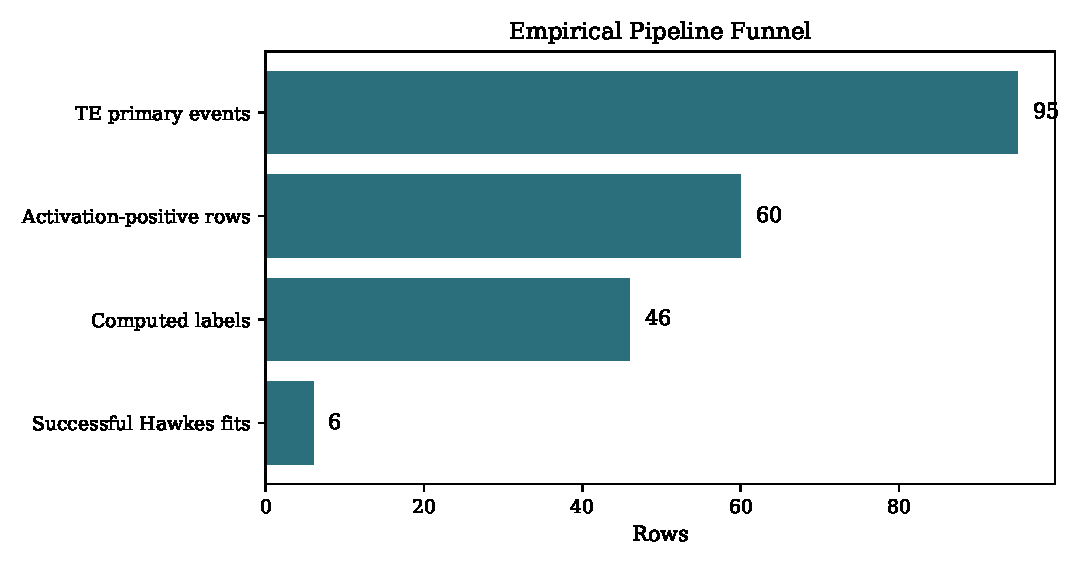
\includegraphics[width=0.92\textwidth]{figures/figure_1_pipeline_funnel.pdf}
\caption{Empirical pipeline funnel from primary macro candidates through successful Hawkes fits.}
\label{fig:figure-1}
\end{figure}

\begin{figure}[htbp]
\centering
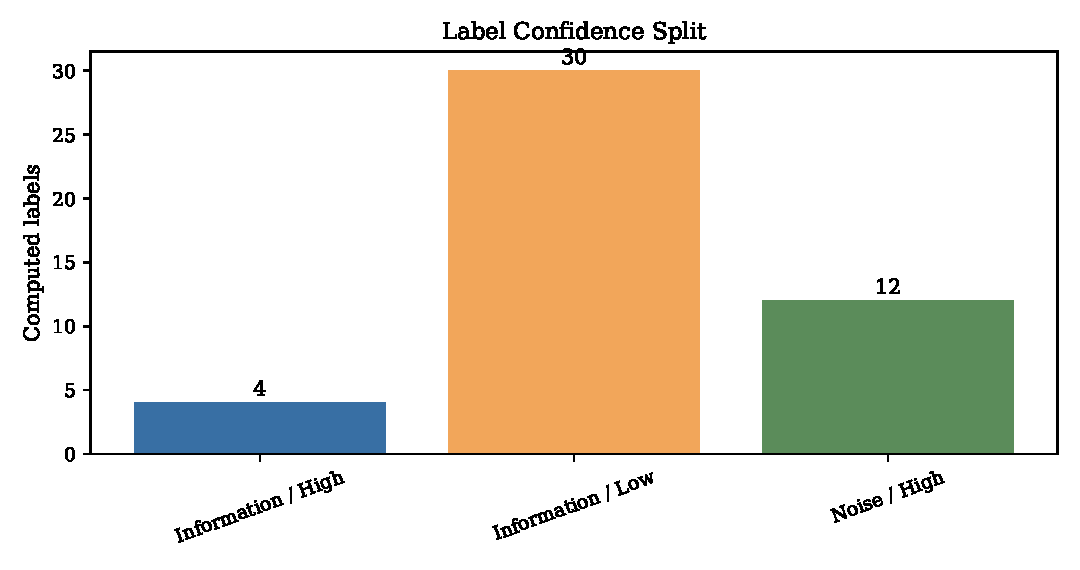
\includegraphics[width=0.92\textwidth]{figures/figure_2_label_confidence_split.pdf}
\caption{Computed label confidence split under the PPI-primary/RR-validator policy.}
\label{fig:figure-2}
\end{figure}

\begin{figure}[htbp]
\centering
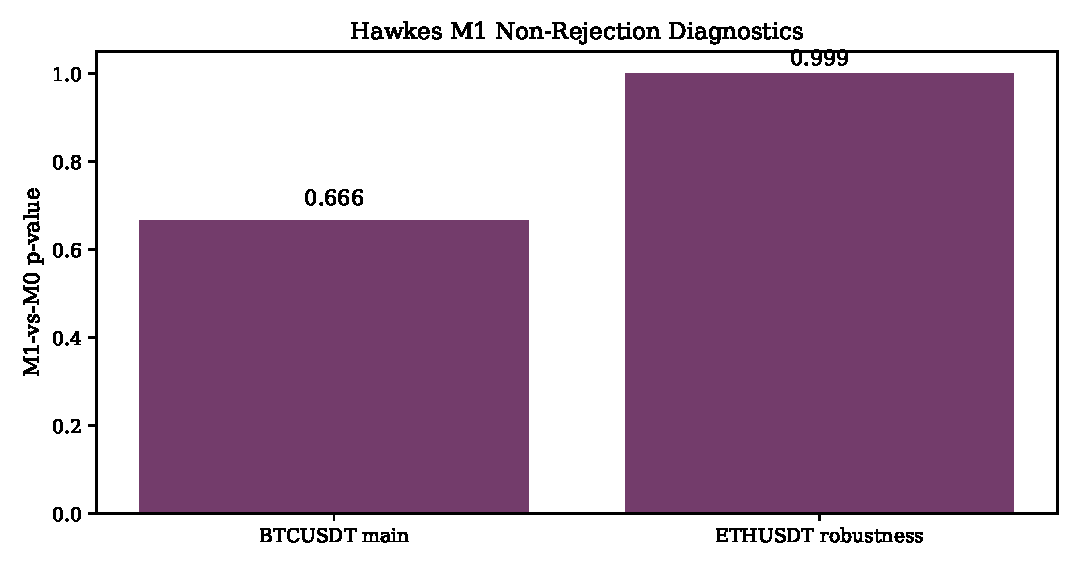
\includegraphics[width=0.92\textwidth]{figures/figure_3_hawkes_m1_pvalues.pdf}
\caption{Nominal M1-vs-M0 p-values for the main and robustness cohorts. Values are shown only as diagnostic summaries of Table 5; no calibrated rejection threshold is plotted because cluster-calibrated thresholds are unavailable at the current cohort-level effective sample (4 release-batch clusters for BTCUSDT main; 3 for ETHUSDT robustness). See Section 6.2 for the diagnostic and Section 6.6 for the three structural barriers behind it.}
\label{fig:figure-3}
\end{figure}
\end{document}
